% TODO:
% 3) Bitmap index, пример














%%%%%%%%%%%%%%%%%%%%%%%%%%%%%%%%%%%%%%%%%
% Beamer Presentation
% LaTeX Template
% Version 1.0 (10/11/12)
%
% This template has been downloaded from:
% http://www.LaTeXTemplates.com
%
% License:
% CC BY-NC-SA 3.0 (http://creativecommons.org/licenses/by-nc-sa/3.0/)
%
%%%%%%%%%%%%%%%%%%%%%%%%%%%%%%%%%%%%%%%%%

%----------------------------------------------------------------------------------------
%	PACKAGES AND THEMES
%----------------------------------------------------------------------------------------

\documentclass[compress, dvipsnames, unicode]{beamer}

\mode<presentation> {

% The Beamer class comes with a number of default slide themes
% which change the colors and layouts of slides. Below this is a list
% of all the themes, uncomment each in turn to see what they look like.

%\usetheme{default}
%\usetheme{AnnArbor}
%\usetheme{Antibes}
%\usetheme{Bergen}
%\usetheme{Berkeley}
%\usetheme{Berlin}
%\usetheme{Boadilla}
%\usetheme{CambridgeUS}
%\usetheme{Copenhagen}
%\usetheme{Darmstadt}
%\usetheme{Dresden}
%\usetheme{Frankfurt}
%\usetheme{Goettingen}
%\usetheme{Hannover}
%\usetheme{Ilmenau}
%\usetheme{JuanLesPins}
%\usetheme{Luebeck}
\usetheme{Madrid}
%\usetheme{Malmoe}
%\usetheme{Marburg}
%\usetheme{Montpellier}
%\usetheme{PaloAlto}
%\usetheme{Pittsburgh}
%\usetheme{Rochester}
%\usetheme{Singapore}
%\usetheme{Szeged}
%\usetheme{Warsaw}

% As well as themes, the Beamer class has a number of color themes
% for any slide theme. Uncomment each of these in turn to see how it
% changes the colors of your current slide theme.

%\usecolortheme{albatross}
%\usecolortheme{beaver}
%\usecolortheme{beetle}
%\usecolortheme{crane}
%\usecolortheme{dolphin}
%\usecolortheme{dove}
%\usecolortheme{fly}
%\usecolortheme{lily}
%\usecolortheme{orchid}
%\usecolortheme{rose}
%\usecolortheme{seagull}
%\usecolortheme{seahorse}
%\usecolortheme{whale}
%\usecolortheme{wolverine}

%\setbeamertemplate{footline} % To remove the footer line in all slides uncomment this line
%\setbeamertemplate{footline}[page number] % To replace the footer line in all slides with a simple slide count uncomment this line

%\setbeamertemplate{navigation symbols}{} % To remove the navigation symbols from the bottom of all slides uncomment this line
}

\beamertemplatenavigationsymbolsempty

\usepackage{customPackage}

\usepackage[]{algorithmicx}
\usepackage[noend]{algpseudocode}
\usepackage{rotating}

\usepackage{pgfplots}
\usepackage{pgfmath,pgffor}
\pgfplotsset{compat=newest}
\usepackage{adjustbox}
\usepackage{xcolor}
\usepackage[first=0, last=2]{lcg}
\usepackage{multirow}

\usepackage{listings}
\lstset{
    literate={~} {$\sim$}{1},
    basicstyle=\ttfamily,
    numbers=left,
    xleftmargin=2.5em,
    framexleftmargin=2em,
    frame=single,
    captionpos=b,
}


\usepackage{amsmath, amsfonts, graphicx}
\usepackage{cases}
\usepackage{tikz,tcolorbox}
\usetikzlibrary{shapes,calc, arrows.meta}
\usetikzlibrary{matrix,backgrounds}
\usetikzlibrary{positioning}
\tcbuselibrary{skins}

\tikzstyle{stnode} = [
circle,
draw=blue,
thick,
fill=blue!20,
minimum width=0.1em,
%minimum height=2em
]

\usepackage[utf8]{inputenc}
\usepackage[russian]{babel}
\usepackage{cmap}
\usepackage{subcaption}
\usepackage[]{algorithmicx}
\usepackage[noend]{algpseudocode}
\usepackage{verbatim}
\usepackage{fancybox}
\usepackage{ulem}
\usepackage{tikz}
\usetikzlibrary{positioning}
\usepackage{scalefnt}
\usetikzlibrary{arrows,shapes,positioning,shadows,trees,calc,backgrounds,fit,positioning}

\usepackage{graphicx} % Allows including images
\graphicspath{{images/}}
\usepackage{booktabs} % Allows the use of \toprule, \midrule and \bottomrule in tables
\usepackage{textcomp}
\usepackage{listings}
\usepackage{color}
\usepackage{xcolor,colortbl}
\usepackage{changepage}
\usepackage{array}

\newcolumntype{L}[1]{>{\raggedright\let\newline\\\arraybackslash\hspace{0pt}}m{#1}}
\newcolumntype{C}[1]{>{\centering\let\newline\\\arraybackslash\hspace{0pt}}m{#1}}
\newcolumntype{R}[1]{>{\raggedleft\let\newline\\\arraybackslash\hspace{0pt}}m{#1}}


\usepackage{pgfplots}
\usepackage{pgfmath,pgffor}
\pgfplotsset{compat=newest}
\usepackage{adjustbox}
\usepackage[first=0, last=2]{lcg}

\definecolor{mygreen}{rgb}{0,0.6,0}
\definecolor{mygray}{rgb}{0.5,0.5,0.5}
\definecolor{mymauve}{rgb}{0.58,0,0.82}

\lstset{ %
	backgroundcolor=\color{white},   % choose the background color; you must add \usepackage{color} or \usepackage{xcolor}
	basicstyle=\footnotesize,        % the size of the fonts that are used for the code
	breakatwhitespace=false,         % sets if automatic breaks should only happen at whitespace
	breaklines=true,                 % sets automatic line breaking
	captionpos=b,                    % sets the caption-position to bottom
	commentstyle=\color{mygreen},    % comment style
	deletekeywords={...},            % if you want to delete keywords from the given language
	escapeinside={\%*}{*)},          % if you want to add LaTeX within your code
	extendedchars=true,              % lets you use non-ASCII characters; for 8-bits encodings only, does not work with UTF-8
	frame=single,                    % adds a frame around the code
	keepspaces=true,                 % keeps spaces in text, useful for keeping indentation of code (possibly needs columns=flexible)
	keywordstyle=\color{blue},       % keyword style
	language=Octave,                 % the language of the code
	morekeywords={*,...},            % if you want to add more keywords to the set
	numbers=left,                    % where to put the line-numbers; possible values are (none, left, right)
	numbersep=5pt,                   % how far the line-numbers are from the code
	numberstyle=\tiny\color{mygray}, % the style that is used for the line-numbers
	rulecolor=\color{black},         % if not set, the frame-color may be changed on line-breaks within not-black text (e.g. comments (green here))
	showspaces=false,                % show spaces everywhere adding particular underscores; it overrides 'showstringspaces'
	showstringspaces=false,          % underline spaces within strings only
	showtabs=true,                  % show tabs within strings adding particular underscores
	stepnumber=1,                    % the step between two line-numbers. If it's 1, each line will be numbered
	stringstyle=\color{mymauve},     % string literal style
	tabsize=4,                       % sets default tabsize to 2 spaces
	%title=\lstname                   % show the filename of files included with \lstinputlisting; also try caption instead of title
}

%----------------------------------------------------------------------------------------
%	TITLE PAGE
%----------------------------------------------------------------------------------------

\title[PosDB~--- a distributed column-store]{PosDB~--- a distributed column-store with late materialization
} % The short title appears at the bottom of every slide, the full title is only on the title page

\author{George Chernishev} % Your name
\institute[] % Your institution as it will appear on the bottom of every slide, may be shorthand to save space
{
Saint-Petersburg State University,\\
National Research University Higher School of Economics\\

\medskip
\textit{chernishev@gmail.com} % Your email address
}
%\date{\today} % Date, can be changed to a custom date

\date{December 2019}

\begin{document}

\begin{frame}
\titlepage % Print the title page as the first slide
\end{frame}

\begin{comment}
\begin{frame}
\frametitle{Overview} % Table of contents slide, comment this block out to remove it
\tableofcontents % Throughout your presentation, if you choose to use \section{} and \subsection{} commands, these will automatically be printed on this slide as an overview of your presentation
\end{frame}
\end{comment}

\begin{frame}{Scope}

\begin{itemize}
\setlength\itemsep{0.5em}
\item Column-oriented query processing
\item Late materialization overview
\item Existing systems and PosDB Motivation
\item Query plans in PosDB
\item Data acquisition: access methods and data readers
\item PosDB as a research platform
\item Conclusion: team, state, future plans
\end{itemize}
\end{frame}

\begin{frame}{Column-store: an idea}
\begin{itemize}
	\item Data is stored in columns, not in rows:
\end{itemize}
\begin{columns}
	\begin{column}{0.35\textwidth}
		\begin{adjustbox}{max width=1.0\textwidth}
			\begin{tikzpicture}[
	line/.style={
	draw,
	-{Stealth[length=2mm]},
},]
    \tikzstyle{every node} = [rectangle,draw, fill=blue!30, minimum height=18pt]
    \node[](A0){Name};
    \node[right=0pt of A0](B0){Type};
    \node[right=0pt of B0](C0){Year};
    \node[right=0pt of C0](D0){Month};
    \node[right=0pt of D0](E0){Day};
    
    \foreach \i in {1, ..., 4} {
        \pgfmathtruncatemacro{\pred}{\i - 1}
        
        \ifthenelse{\i = 1} {
            \node[below right=5pt and -25pt of A\pred](A\i){\phantom{Name}};
        } {
        \node[below right=-7pt and -25pt of A\pred](A\i){\phantom{Name}};
    }
    \node[right=0pt of A\i](B\i){\phantom{Type}};
    \node[right=0pt of B\i](C\i){\phantom{Year}};
    \node[right=0pt of C\i](D\i){\phantom{Month}};
    \node[right=0pt of D\i](E\i){\phantom{Day}};
		\draw[line] ($(A0.north west) + (0, 0.3)$) -- ($(E0.north east) + (0, 0.3)$);  
}
\end{tikzpicture}			
		\end{adjustbox}
	\end{column}%%%%
	\begin{column}{0.47\textwidth}
		\begin{adjustbox}{max width=1.0\textwidth}
			\begin{tikzpicture}[
	line/.style={
	draw,
	-{Stealth[length=2mm]},
},]
\tikzstyle{every node} = [rectangle,draw, fill=orange!50, minimum height=18pt]
\node[](A0){Name};
\node[right=10pt of A0](B0){Type};
\node[right=10pt of B0](C0){Year};
\node[right=10pt of C0](D0){Month};
\node[right=10pt of D0](E0){Day};

\foreach \i in {1, ..., 4} {
    \pgfmathtruncatemacro{\pred}{\i - 1}
    
    \ifthenelse{\i = 1} {
        \node[below right=5pt and -28pt of A\pred](A\i){\phantom{Name}};
    } {
    \node[below right=-7pt and -28pt of A\pred](A\i){\phantom{Name}};
}
\node[right=10pt of A\i](B\i){\phantom{Type}};
\node[right=10pt of B\i](C\i){\phantom{Year}};
\node[right=10pt of C\i](D\i){\phantom{Month}};
\node[right=10pt of D\i](E\i){\phantom{Day}};
\draw[line] ($(A0.north west) + (-0.5, 0)$) -- ($(A0.north west) + (0.6, -2.75)$);  
}
\end{tikzpicture}

		\end{adjustbox}
	\end{column}
\end{columns}
\vspace{3mm}
\begin{itemize}
	\item Only requested columns is read;
	\item Efficient use of hardware, e.g. vectorization.
\end{itemize}
\vspace{3mm}
Column-stores:
\begin{itemize}
	\item[+] Excel at handling read-only queries, useful for handling OLAP;
	\item[+] Also popular in recently emerged HTAP applications;
	\item[--] Updates are costly, HDD-based OLTP suffers.
\end{itemize}

\end{frame}


\begin{frame}{Columnar approach: contemporary view}

Nowadays many industrial systems call themselves ``columnar''.\\~\\

They treat column-orientation as storage level-only:
\begin{itemize}
	\setlength\itemsep{0.5em}		
	\item processing is usually organized as follows: ``read, decompress data,\\ construct tuples, continue to work as usual'';
    \item allows to read only requested columns;
	\item efficient column-oriented compression.
\end{itemize}

\end{frame}

\begin{frame}{Columnar approach: founders vision}

However, founders proposed not only column-oriented data \textbf{\textit{storage}}, but also column-oriented data \textbf{\textit{processing}}:

\begin{itemize}	
    \item query plans allow operators exchange not only data, but also positions;
    \item an option to select tuple reconstruction time: transition from positions to records
	\begin{itemize}
		\item early materialization
		\item late materialization
	\end{itemize}
	\item operating directly on compressed data.
\end{itemize}
$\longrightarrow$ novel operators, novel query plans.

\end{frame}

\begin{frame}
\frametitle{Query execution: EM example}

\begin{figure}[htb]
	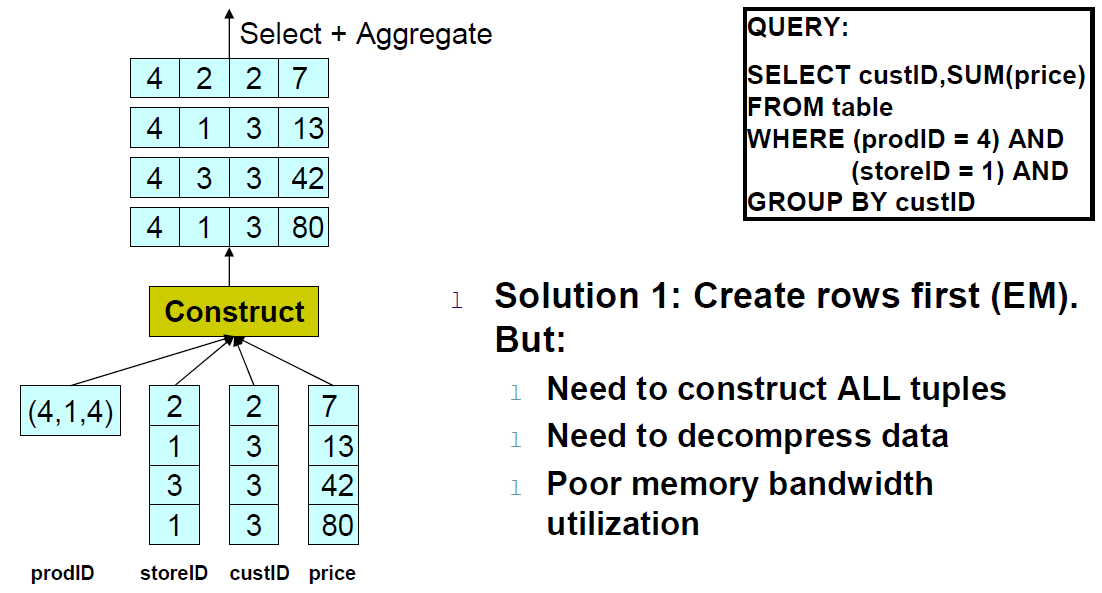
\includegraphics[width=\textwidth,height=0.75\textheight,keepaspectratio]{em.png} 
	\footnote{\tiny{Image is taken from D. Abadi, P. Boncz, and S. Harizopoulos. Column-oriented database systems. Proc. VLDB Endow. 2, 2 (August 2009)}}
\end{figure}    

\end{frame}

\begin{frame}
\frametitle{Query execution: LM example I}

\begin{figure}[htb]
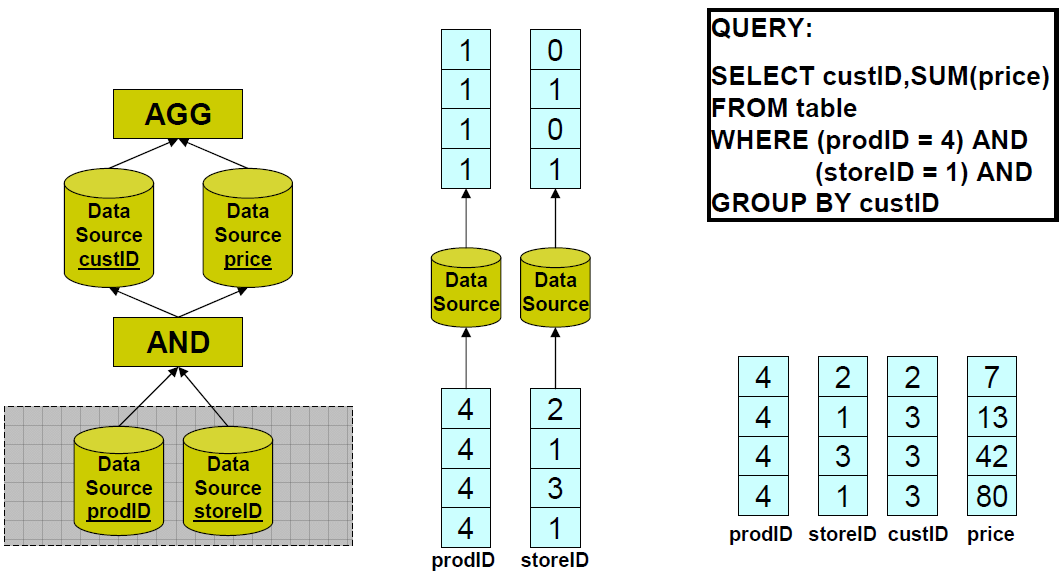
\includegraphics[width=\textwidth,height=0.75\textheight,keepaspectratio]{lm1.png} 
\footnote{\tiny{Image is taken from D. Abadi, P. Boncz, and S. Harizopoulos. Column-oriented database systems. Proc. VLDB Endow. 2, 2 (August 2009)}}
\end{figure}    

\end{frame}

\begin{frame}
\frametitle{Query execution: LM example II}

\begin{figure}[htb]
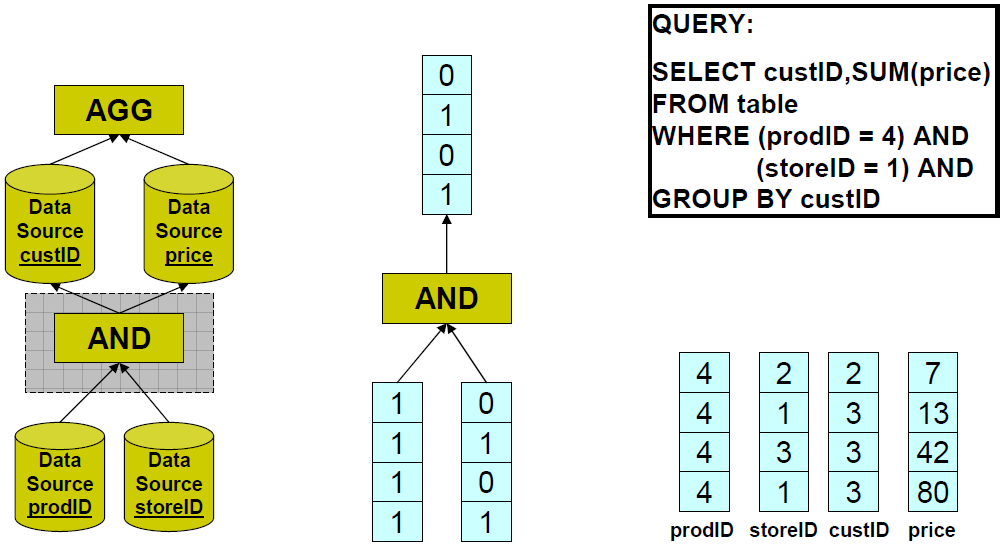
\includegraphics[width=\textwidth,height=0.75\textheight,keepaspectratio]{lm2.png} 
\footnote{\tiny{Image is taken from D. Abadi, P. Boncz, and S. Harizopoulos. Column-oriented database systems. Proc. VLDB Endow. 2, 2 (August 2009)}}
\end{figure}    

\end{frame}

\begin{frame}
\frametitle{Query execution: LM example III}

\begin{figure}[htb]
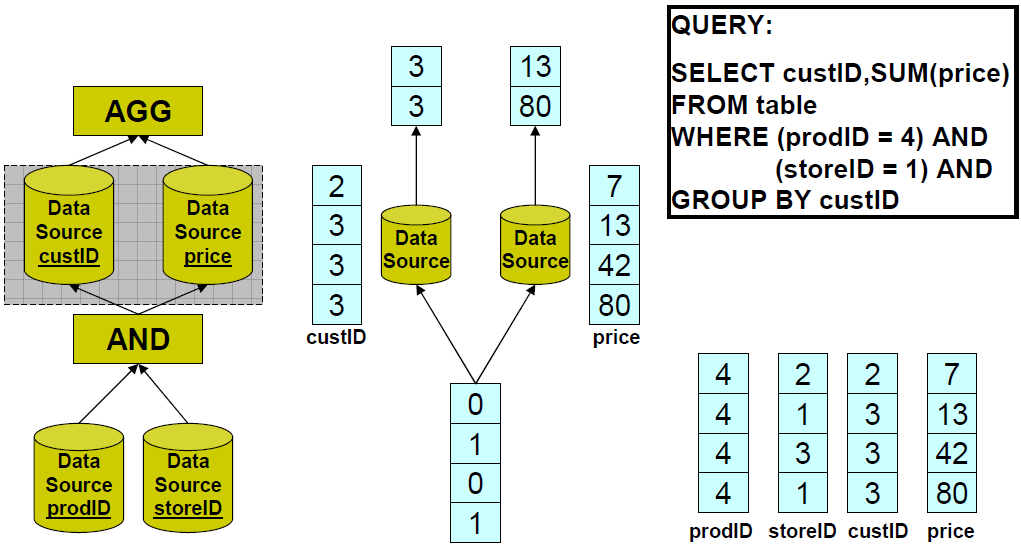
\includegraphics[width=\textwidth,height=0.75\textheight,keepaspectratio]{lm3.png} 
\footnote{\tiny{Image is taken from D. Abadi, P. Boncz, and S. Harizopoulos. Column-oriented database systems. Proc. VLDB Endow. 2, 2 (August 2009)}}
\end{figure}    

\end{frame}

\begin{frame}
\frametitle{Query execution: LM example IV}

\begin{figure}[htb]
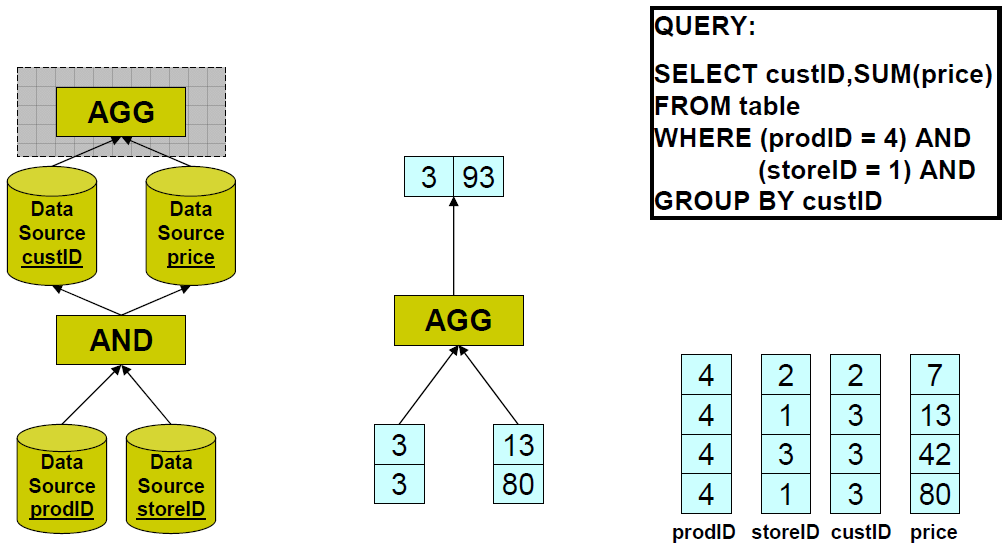
\includegraphics[width=\textwidth,height=0.75\textheight,keepaspectratio]{lm4.png} 
\footnote{\tiny{Image is taken from D. Abadi, P. Boncz, and S. Harizopoulos. Column-oriented database systems. Proc. VLDB Endow. 2, 2 (August 2009)}}
\end{figure}    

\end{frame}


\begin{frame}{Existing column-stores}
\begin{center}	
	\begin{tabular}{l | C{3.5cm} | C{2.5cm} | C{2.5cm} }
		\hline
		System & Centralized or distributed & Sources Available? & Disk-based or in-memory? \\\hline
		C-Store 	& \multirow{2}{*}{Centralized}  & \cellcolor{Green} & Disk-based \\
		MonetDB 	&   & \multirow{-2}{*}{\cellcolor{Green} Yes}  & in-memory \\\hline
		
		Vertica 	& \multirow{2}{*}{Distributed} 	& \cellcolor{Red} & Disk-based \\
		Vector 		&   	& \multirow{-2}{*}{\cellcolor{Red} No} & Disk-based with in-memory tuning \\\hline
		
		ScaMMDB 	& \multirow{2}{*}{Distributed} 	& \cellcolor{Red} & \multirow{2}{*}{in-memory} \\
		DCODE   	&  & \multirow{-2}{*}{\cellcolor{Red} No} &  \\\hline
		
		ClickHouse 	& Distributed 	& \cellcolor{Green} Yes & Disk-based \\\hline
	\end{tabular}
\end{center}

\ldots and a lot of other commercial (mostly centralized) systems.

% Голосом можно сказать, что речь здесь только о реляционных СУБД.
\end{frame}

\begin{frame}{Motivation behind PosDB}
	\begin{itemize}
	    \item Studies related to many problems were not finished: aggregation, subqueries, \ldots
		\item Distributed processing for column-stores is not studied, ScaMMDB and DCODE projects are abandoned
	\end{itemize}
	\begin{center}
		{\LARGE $\Downarrow$}\\
		Need a prototype of a new distributed column-store
	\end{center}

	\begin{itemize}
		\item Since \textbf{\textit{disk-based}} distributed column-stores were not studied at all, we decided to concentrate on this type.
	\end{itemize}
\end{frame}

% \begin{frame}{Why developing from scratch}
% 	\begin{itemize}
% 		\setlength\itemsep{0.5em}
% 		\item There are only two open-sourced disk-based column-stores:
% 		\begin{itemize}
% 			\item C-Store~--- low quality of code in available version, cant build the system even in original environment, project is closed.
% 			\item ClickHouse~--- a very active project:
% 			\begin{itemize}
% 				\item non-standard architecture
% 				\item new terminology for classic stuff
% 				\item poor module decomposition, spaghetti code
% 				\item no late materialization
% 			\end{itemize}
% 		\end{itemize}
% 		\item Therefore, basing on an existing system would have forced us to deal with lots of issues and lead to a number of limitations. Eventually, it would not have been beneficial at all.
% 	\end{itemize}
% \end{frame}

\begin{frame}{PosDB}
A distributed disk-based column-store for research purposes:
\vspace{0.3em}
\begin{itemize}
	\setlength\itemsep{0.5em}
	\item Relies on Volcano block-based iterator model.
	\item \underline{Columnar}: operators exchange not only data, but also positions (\alert{PosDB}).
	\item \underline{Disk-based}: data $>>$ main memory.
	\item \underline{Distributed}: has send \& receive operators.
	Not mediator-based, but ``true'' distribution of data and queries.
	\item \underline{Parallel}: any operator sub-tree can be executed in a separate thread.
	\item Currently relies on \underline{late materialization}, however, recently elements of \underline{hybrid materialization} were added.
\end{itemize}
\end{frame}

\begin{frame}{Query plans, Volcano model, Late materialization}
\begin{figure}
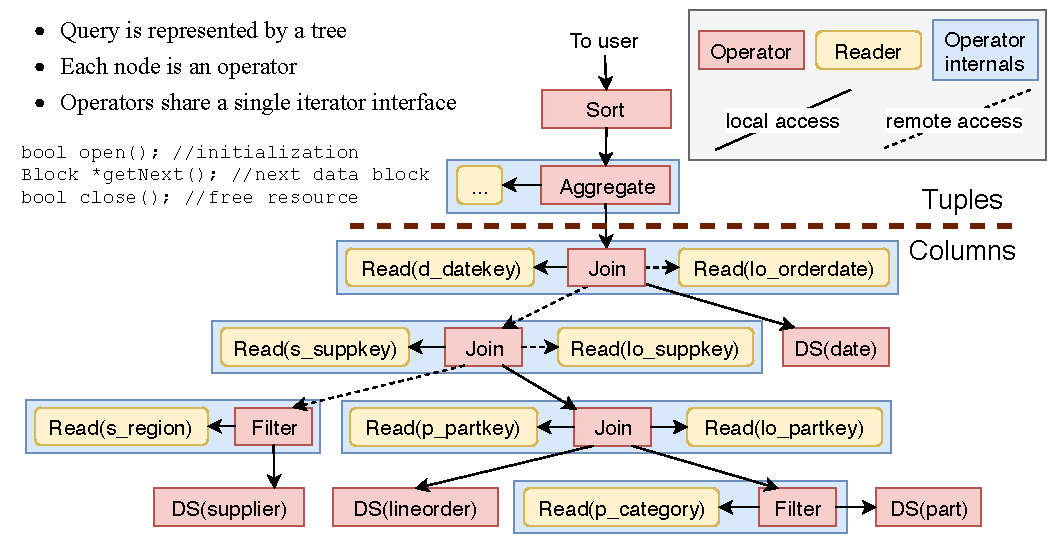
\includegraphics[width=\textwidth,height=\textheight,keepaspectratio]{images/volcano_query.pdf}
\end{figure}
\end{frame}

\begin{frame}{Join index}
\begin{columns}
	\begin{column}{0.52\textwidth}
	    Query may contain joins, therefore a special data block is required:
        \vspace{0.5em}
        
		\begin{itemize}
		\setlength\itemsep{1em}
			\item Use classic data structure;
			\item Position lists, one per table;
			\item Two tables: a map of positions of $T_1$ into positions of $T_2$;
			\item $N$ tables: a map of positions of $T_1, T_2, T_{N-1}$ into positions of $T_N$
		\end{itemize}	
	\end{column}%%
	\begin{column}{0.43\textwidth}
	\begin{figure}
	    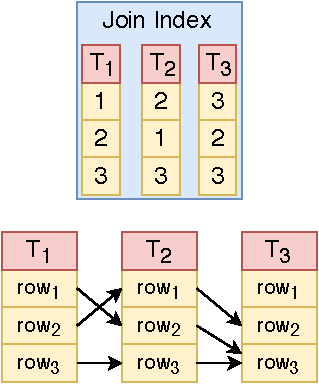
\includegraphics[width=0.9\textwidth]{images/join_index.pdf}
	\end{figure}
	\end{column}
\end{columns}	
\end{frame}

\begin{frame}[fragile]{Acquiring data and positions}
\begin{columns}
\begin{column}{0.63\textwidth}
\begin{enumerate}
	\setlength\itemsep{1em}
	\item Initial \texttt{JoinIndex} acquisition happens in leaves of a tree via \texttt{DataSource} operator
	\item All necessary data is read inside operators
\end{enumerate}
\end{column}
\begin{column}{0.3\textwidth}
\begin{tikzpicture}[
column/.style={
	rectangle,
	draw=Purple,
	thick,
	fill=Dandelion!90,
	text width=6.7em,
	align=center,
	%		minimum height=0.6em,
},
block/.style={
	rectangle,
	draw=blue,
	thick,
	fill=blue!20,
	text width=7.5em,
	align=center,
	rounded corners,
	minimum height=3.5em
},]
\draw (0,0) node[block](N5){};
\path (0,0.37) node[] (N1) {Operator}
(0,-0.23) node[column] (N2) {Data reading}
(0.15,-1) node[] (N3) {\textit{positions}}
(0.15,0.875) node[] (N4) {\textit{positions}};
\draw[-{Stealth[length=2mm, width=1.5mm]}] ($(N5.north) +(-0.7,0)$) -- ($(N5.north) + (-0.7,0.5)$);  
\draw[-{Stealth[length=2mm, width=1.5mm]}] ($(N5.south) +(-0.7,-0.45)$) -- ($(N5.south) + (-0.7,0)$);  
\end{tikzpicture}
\end{column}
\end{columns}
%\vspace{1em}
\begin{figure}[htb]
\begin{tikzpicture}[
 	column/.style={
 		rectangle,
 		draw=Purple,
 		thick,
 		fill=Dandelion!90,
 		text width=6.7em,
 		align=center,
 		%		minimum height=0.6em,
 	},
 	block/.style={
 		rectangle,
 		draw=blue,
 		thick,
 		fill=blue!20,
 		text width=7.5em,
 		align=center,
 		rounded corners,
 		minimum height=3.5em
 	},
 block2/.style={
 	rectangle,
 	draw=blue,
 	thick,
 	fill=blue!20,
 	text width=7em,
 	align=center,
 	rounded corners,
 	minimum height=1.5em
 },
-{Stealth[length=2mm, width=1.5mm]}]
 	\draw (0,-0.2) node[column](N1){Data reading};
 	\path (-3,-1) node[column] (N2) {Remote}
 	(3,-1) node[column] (N3) {Local}
 	(-3,-1.9) node[block2] (N4) {NetworkReader}
 	(-3,-3.3) node[block2] (N5) {RemoteReader}
 	(3,-1.9) node[block2] (N6) {XXXReader}
 	(3,-3.3) node[block2] (N7) {Disk}
 	;
 	\draw (N1) -- (N2.east);
  	\draw (N1) -- (N3.west);
  	\draw[{Stealth[length=2mm, width=1.5mm]}-{Stealth[length=2mm, width=1.5mm]}] (N4.south east) -- (N5.north east) node [midway, left] {Network}; 
  	\draw[{Stealth[length=2mm, width=1.5mm]}-{Stealth[length=2mm, width=1.5mm]}] (N6.south west) -- (N7.north west) node [midway, right] {Storage subsystem}; 
 	\end{tikzpicture}
\end{figure}
\end{frame}

\begin{frame}{Data access}
\begin{itemize}
    \item \textbf{Reader}: global strategy to get data for a position \textit{stream}
    \item \textbf{Access method}: \textit{local} access to data for a position \textit{block}
\end{itemize}
\vspace{1em}

\begin{figure}[htb]

	\definecolor{reader}{HTML}{ffeda0}%
	\begin{tikzpicture}[
	block/.style={
		rectangle,
		draw=black,
		thick,
		align=center,
	},
	-{Stealth[length=2mm, width=1.5mm]}]
	\draw (0em,0em) node[block, fill=reader, minimum height=5em, text width=9em](N){};
	\path (0,-0.25) node[] (N1) {\Large Storage System}
	(0,-1.225) node[block,fill=blue!20, text width=9em] (N2) {Disk}
	(0,0.68) node[block, fill=Dandelion!90,] (N4) {Access methods}
	(3.5,0.7) node[block] (N5) {AccessRange\\ AccessSorted\\ AccessJive}
	(0,2) node[block, fill=Dandelion!90,] (N6) {RangeReader SortedReader JiveReader}
	;
	\draw[densely dashed] (N4) -- (N5);
	\draw[{Stealth[length=2mm, width=1.5mm]}-{Stealth[length=2mm, width=1.5mm]}] (N4) -- (N6) node [midway, left] {Blocks of data};  
	\end{tikzpicture}
\end{figure}
\end{frame}

\begin{frame}{Access methods}
For a position block access data \textit{efficiently}:
\vspace{0.3em}

\begin{enumerate}
\setlength\itemsep{0.5em}
    \item contiguous position range (\texttt{AccessRange}): \texttt{for} loop, sequential pages
    \item sparse sorted list of positions (\texttt{AccessSorted}): similar to \texttt{for} loop, page number always increasing (one-direction file read)
    \item sparse unordered list of positions (\texttt{AccessJive}) -- ?
\end{enumerate}
\vspace{1.5em}

% \texttt{AccessJive}:
% \begin{enumerate}
%     \item Sort position list
%     \item Read data efficiently
%     \item Sort both positions and data backwards
% \end{enumerate}
    
\begin{adjustbox}{max width=\textwidth}
\begin{tikzpicture}[->,
]
\tikzset{
	/mycolumn/box/.style={draw=black, fill=orange!80},
	/mycolumn/text/.style={font=\small},
	/mycolumn/width=0.5,
	/mycolumn/height=0.5,
}
\datacolumn[name=init1]{0}{0}{3,11,7,5,9}

\datacolumn[name=pseudo1, box/.append style={fill=orange!30, dashed}]{2}{0}{1,2,3,4,5}
\datacolumn[name=init2]{2.75}{0}{3,11,7,5,9}

\datacolumn[name=pseudo2, box/.append style={fill=orange!30, dashed}]{4.75}{0}{1,4,3,5,2}
\datacolumn[name=init3]{5.5}{0}{3,5,7,9,11}

\datacolumn[name=pseudo3, box/.append style={fill=orange!30, dashed}]{7.5}{0}{1,4,3,5,2}
\datacolumn[name=init4]{8.25}{0}{3,5,7,9,11}
\datacolumn[name=data1, width=1.25, box/.append style={fill=LimeGreen}]{9.25}{0}{Aus, Noch, Zu, Sonst, Neun}

\datacolumn[name=pseudo4, box/.append style={fill=orange!30, dashed}]{11.625}{0}{1,2,3,4,5}
\datacolumn[name=init5]{12.375}{0}{3,11,7,5,9}
\datacolumn[name=data2, width=1.25, box/.append style={fill=LimeGreen}]{13.375}{0}{Aus, Neun, Zu, Noch, Sonst}

\draw ($(init12.east) + (0.15,0)$) -- node [above,midway, text width=2.5em, align=center] {Save Order} ($(pseudo12.west) - (0.15, 0)$);
\draw ($(init22.east) + (0.15,0)$) -- node [above,midway, text width=2.5em, align=center] {Re- order} ($(pseudo22.west) - (0.15, 0)$);
\draw ($(init32.east) + (0.15,0)$) -- node [above,midway, text width=2.5em, align=center] {Read data} ($(pseudo32.west) - (0.15, 0)$);
\draw ($(data12.east) + (0.15,0)$) -- node [above,midway, text width=2.5em, align=center] {Re- order} ($(pseudo42.west) - (0.15, 0)$);
\end{tikzpicture}
	
\end{adjustbox}

\end{frame}

% \begin{frame}{AccessJive: idea}
% \centering
% \begin{adjustbox}{max width=\textwidth}
% \begin{tikzpicture}[->,
]
\tikzset{
	/mycolumn/box/.style={draw=black, fill=orange!80},
	/mycolumn/text/.style={font=\small},
	/mycolumn/width=0.5,
	/mycolumn/height=0.5,
}
\datacolumn[name=init1]{0}{0}{3,11,7,5,9}

\datacolumn[name=pseudo1, box/.append style={fill=orange!30, dashed}]{2}{0}{1,2,3,4,5}
\datacolumn[name=init2]{2.75}{0}{3,11,7,5,9}

\datacolumn[name=pseudo2, box/.append style={fill=orange!30, dashed}]{4.75}{0}{1,4,3,5,2}
\datacolumn[name=init3]{5.5}{0}{3,5,7,9,11}

\datacolumn[name=pseudo3, box/.append style={fill=orange!30, dashed}]{7.5}{0}{1,4,3,5,2}
\datacolumn[name=init4]{8.25}{0}{3,5,7,9,11}
\datacolumn[name=data1, width=1.25, box/.append style={fill=LimeGreen}]{9.25}{0}{Aus, Noch, Zu, Sonst, Neun}

\datacolumn[name=pseudo4, box/.append style={fill=orange!30, dashed}]{11.625}{0}{1,2,3,4,5}
\datacolumn[name=init5]{12.375}{0}{3,11,7,5,9}
\datacolumn[name=data2, width=1.25, box/.append style={fill=LimeGreen}]{13.375}{0}{Aus, Neun, Zu, Noch, Sonst}

\draw ($(init12.east) + (0.15,0)$) -- node [above,midway, text width=2.5em, align=center] {Save Order} ($(pseudo12.west) - (0.15, 0)$);
\draw ($(init22.east) + (0.15,0)$) -- node [above,midway, text width=2.5em, align=center] {Re- order} ($(pseudo22.west) - (0.15, 0)$);
\draw ($(init32.east) + (0.15,0)$) -- node [above,midway, text width=2.5em, align=center] {Read data} ($(pseudo32.west) - (0.15, 0)$);
\draw ($(data12.east) + (0.15,0)$) -- node [above,midway, text width=2.5em, align=center] {Re- order} ($(pseudo42.west) - (0.15, 0)$);
\end{tikzpicture}
	
% \end{adjustbox}
% \end{frame}

% \begin{frame}{Query Plan: example}
% \begin{figure}[htb]
% 	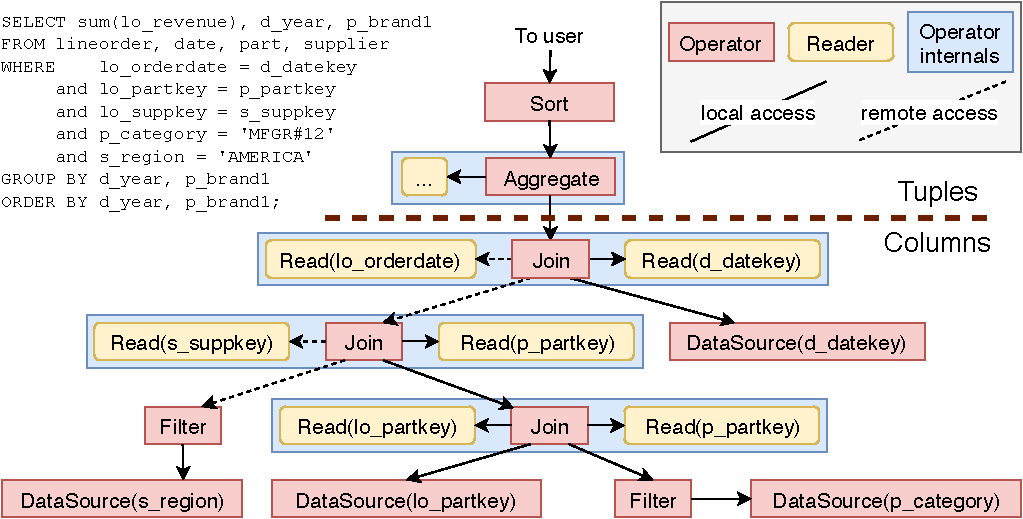
\includegraphics[width=\textwidth,height=0.80\textheight,keepaspectratio]{query.pdf} 
% \end{figure}
% \end{frame}

\begin{frame}{Mixed stream of positions}
What if stream of positions is local but heterogeneous?
\\~\\
\begin{itemize}
\item Select an optimal access method for each individual block (dynamically)
\item \texttt{AccessJive} worse \texttt{AccessSorted} worse \texttt{AccessRange}
\end{itemize}
\vspace{1em}
\centering
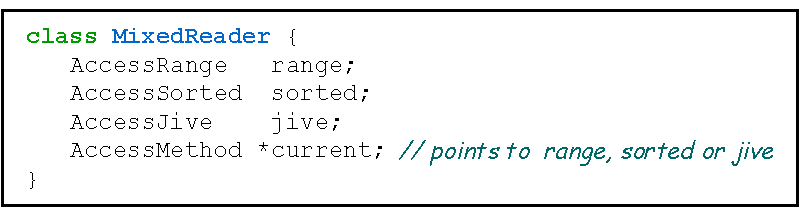
\includegraphics[width=0.9\textwidth]{images/access_jive.pdf} 
\end{frame}

\begin{frame}{Current State}
(+)
\begin{itemize}
\item Supports Star Schema Benchmark;
\item Distribution and parallelism on a plan level:
\begin{itemize}
    \item Both inter- and intra- query parallelism;
    \item Both data fragmentation and replication;
    \item Distributed operators;
\end{itemize}

\item Lots of positional- and value- operators;
\item Recently implemented buffer manager;
\end{itemize}

(--)
\begin{itemize}
\item Up until recently we concentrated on query executor; no rewriter and query optimizer, statistics subsystem;
\item (Mostly) No compression;
\item No vectorized primitives and expression compilation;
\item (Mostly) Late materialization;
\end{itemize}
\end{frame}


\begin{frame}{PosDB as a research platform}

Currently, PosDB is used as a research platform for studying various query processing aspects, e.g.:

    \begin{itemize}
        %\setlength\itemsep{1em}		
        \item Distributed operators: 
        \begin{itemize}
            \item distributed join 
            \item distributed aggregation
        \end{itemize}
        \item Aggregation:
        \begin{itemize}
            \item on-the-fly filtering of groups
            \item window functions
        \end{itemize}
        \item Caching of intermediates
        \item ...
    \end{itemize}
\end{frame}


\begin{frame}{Distributed operations}
\begin{columns}
\begin{column}{0.45\textwidth}
   \begin{center}
       \textbf{\large General idea}
    \end{center}
    \begin{enumerate}
        \item Appropriately distribute data
        \item Compute local intermediates
        \item Merge them to obtain total result
    \end{enumerate}
\end{column}
\begin{column}{0.45\textwidth}
   \begin{center}
       \textbf{\large Problems}
    \end{center}
    \begin{itemize}
        \item Minimize network I/O
        \item Avoid DAG query model
        \item Provide flexible and efficient distributed data model
    \end{itemize}
\end{column}
\end{columns}
\vspace{3em}

\begin{enumerate}
    \item Distributed join: reshuffle, local join, union
    \item Distributed aggregation: decompose, local preaggregate, combine
\end{enumerate}
\end{frame}

\begin{frame}{Distributed join: DAG?}
\centering
\begin{figure}
    \begin{minipage}[c]{0.46\textwidth}
        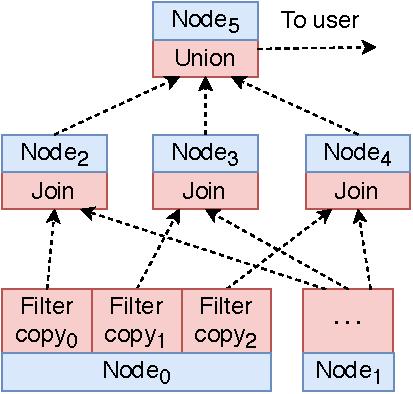
\includegraphics[width=\textwidth]{images/dag_copy.pdf}
        \subcaption{Duplicate approach}
        \label{fig:dag:copy}
    \end{minipage}\hfill
    \begin{minipage}[c]{0.46\textwidth}
        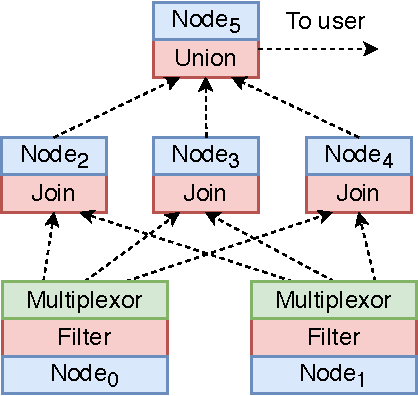
\includegraphics[width=\textwidth]{images/dag_multi.pdf}
        \subcaption{Multiplexor approach}
        \label{fig:dag:multi}
    \end{minipage}
\end{figure}
\end{frame}

\begin{frame}{Multiplexor: 1 to k}
\begin{figure}
    \begin{minipage}[c]{0.04\textwidth}\hfill\end{minipage}%%
    \begin{minipage}[c]{0.5\textwidth}
        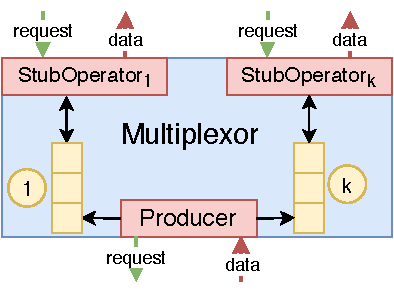
\includegraphics[width=\textwidth]{images/multiplex_arch.pdf}
        \subcaption{Module architecture}
        \label{fig:multiplex:arch}
    \end{minipage}\hfill
    \begin{minipage}[c]{0.34\textwidth}
        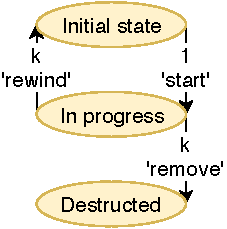
\includegraphics[width=\textwidth]{images/multiplex_state.pdf}
        \subcaption{State diagram}
        \label{fig:multiplex:state}
    \end{minipage}
    \begin{minipage}[c]{0.04\textwidth}\hfill\end{minipage}%%
\end{figure}
\end{frame}

\begin{frame}{Hybrid materialization: optimize network I/O}
\begin{figure}
    \begin{minipage}[c]{0.475\textwidth}
        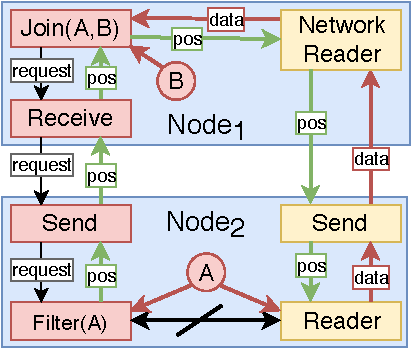
\includegraphics[width=\textwidth]{images/pos_pos_data_1.pdf}
        \subcaption{Late materialization}
    \end{minipage}\hfill
    \begin{minipage}[c]{0.475\textwidth}
        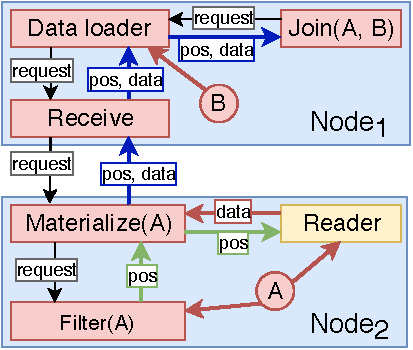
\includegraphics[width=\textwidth]{images/pos_pos_data_3.pdf}
        \subcaption{Hybrid materialization}
    \end{minipage}
    %\caption{PosDB: Join-Filter in a distributed case}
\end{figure}
\end{frame}

\begin{frame}{Distributed aggregation: earlier and now}
\tikzset{
	ds/.style ={
		rectangle,
		draw=red,
		thick,
		fill=red!20,
		minimum width=11.6em,
		align=center,
		rounded corners,
	},
	line/.style={
		draw,
		-{Stealth[length=2mm, width=1.5mm]},
	},
}
\tikzstyle{stnode} = [
rectangle,
draw=blue,
thick,
fill=blue!20,
minimum width=2em,
align=center,
rounded corners
]

\tikzstyle{oldnode} = [
rectangle,
draw=green,
thick,
fill=green!20,
minimum width=2em,
align=center,
rounded corners
]

\tikzstyle{newnode} = [
rectangle,
draw=red,
thick,
fill=red!20,
minimum width=2em,
align=center,
rounded corners
]
	\begin{columns}
		\begin{column}{0.5\linewidth}
			\begin{figure}[ht]
				\centering
				\begin{tikzpicture}[scale=0.7]
				
				\draw (4,-1.5) node[stnode] (N18){UnionAll};
				\path ($(N18) + (0,1.5)$) node[oldnode] (N21) {HGAggregate};
				%\draw[dashed]
				%let \p1=(N21.north),\p2=($(N18.east) + (0.2,0)$) in ($(N18.south west) + (-0.2,-0.2)$) rectangle (\x2,\y1);
				%
				
				%	\draw (-2.25,-3) node[stnode] (N2){ReceivePos};
				\draw (1.875,-3) node[stnode] (N3){ReceivePos};
				\draw (6.125,-3) node[stnode] (N4){ReceivePos};
				%	\draw (10.25,-3) node[stnode] (N5){ReceivePos};
				
				%	\draw[line] (N18.south) -- (N2);
				\draw[line] (N18.south) -- (N3);
				\draw[line] (N18.south) -- (N4);
				%	\draw[line] (N18.south) -- (N5);
				%
				%	\draw (-2.25,-4.5) node[text width=3cm,align=center] (N22){Удаленное поддерево $1$};
				%	\draw[dashed] (N22.north west) rectangle (N22.south east);
				%	\draw[line] (N2) -- (N22.north);
				%
				\draw (1.875,-4.5) node[text width=2.5cm,align=center] (N24){Remote subtree $1$};
				\draw[dashed] (N24.north west) rectangle (N24.south east);
				\draw[line] (N3) -- (N24.north);
				%
				\draw (4,-3) node (N26) {\Large ...};
				\draw[line] (N18) -- (N26.north);
				%
				\draw (6.125,-4.5) node[text width=2.5cm,align=center] (N25){Remote subtree $n$};
				\draw[dashed] (N25.north west) rectangle (N25.south east);
				\draw[line] (N4) -- (N25.north);
				%
				%	\draw (10.25,-4.5) node[text width=3cm,align=center] (N23){Удаленное поддерево $n$};
				%	\draw[dashed] (N23.north west) rectangle (N23.south east);
				%	\draw[line] (N5) -- (N23.north);
				%
				\draw[line] (N21.south) -- (N18);
				\end{tikzpicture}
				%		\caption{Пример распределенного плана с локальной агрегацией}
				%		\label{fig:distributed_plan_with_local_aggregation}
			\end{figure}
		\end{column}
		\begin{column}{0.5\linewidth}
			\begin{figure}[ht]
				\centering
				\begin{tikzpicture}[scale=0.7]
				
				\draw (4,-1.5) node[newnode] (N18){HGCombiner};
				\path ($(N18) + (0,1.5)$) node[newnode] (N21) {Projection};
				%\draw[dashed]
				%let \p1=(N21.north),\p2=($(N18.east) + (0.2,0)$) in ($(N18.south west) + (-0.2,-0.2)$) rectangle (\x2,\y1);
				%
				
				%	\draw (-2.25,-3) node[stnode] (N2){ReceivePos};
				\draw (1.875,-3) node[stnode] (N3){ReceiveTuple};
				\draw (6.125,-3) node[stnode] (N4){ReceiveTuple};
				%	\draw (10.25,-3) node[stnode] (N5){ReceivePos};
				
				%	\draw[line] (N18.south) -- (N2);
				\draw[line] (N18.south) -- (N3);
				\draw[line] (N18.south) -- (N4);
				%	\draw[line] (N18.south) -- (N5);
				%
				%	\draw (-2.25,-4.5) node[text width=3cm,align=center] (N22){Удаленное поддерево $1$};
				%	\draw[dashed] (N22.north west) rectangle (N22.south east);
				%	\draw[line] (N2) -- (N22.north);
				%
				\draw (1.875,-4.5) node[newnode] (N27){HGAggregate};
				\draw (1.875,-6) node[text width=2.5cm,align=center] (N24){Remote subtree $1$};
				\draw[dashed] (N24.north west) rectangle (N24.south east);%\includegraphics[width=0.7\linewidth]{}
				\draw[line] (N3) -- (N27.north);
				\draw[line] (N27) -- (N24.north);
				%
				\draw (4,-3) node (N26) {\Large ...};
				\draw[line] (N18) -- (N26.north);
				%
				\draw (6.125,-4.5) node[newnode] (N28){HGAggregate};
				\draw (6.125,-6) node[text width=2.5cm,align=center] (N25){Remote subtree $n$};
				\draw[dashed] (N25.north west) rectangle (N25.south east);
				\draw[line] (N4) -- (N28.north);
				\draw[line] (N28) -- (N25.north);
				%
				%	\draw (10.25,-4.5) node[text width=3cm,align=center] (N23){Удаленное поддерево $n$};
				%	\draw[dashed] (N23.north west) rectangle (N23.south east);
				%	\draw[line] (N5) -- (N23.north);
				%
				\draw[line] (N21.south) -- (N18);
				\end{tikzpicture}
				%		\caption{Распределенное выполнение агрегации}
				%		\label{fig:distributed_aggregation}
			\end{figure}
		\end{column}
	\end{columns}
\end{frame}

\begin{frame}{Decomposable aggregation functions}
	\begin{block}{Definition (from ``Efficient Evaluation of Aggregates on Bulk Types'')}
		A scalar aggregation function $f: bulk(\tau) \rightarrow \mathcal{N}$ is called \textit{decomposable}, if there exist functions
		\begin{align*}
		\alpha: bulk(\tau)\ &\rightarrow\ \mathcal{N'}\\
		\beta: \mathcal{N'},\ \mathcal{N'}\ &\rightarrow\ \mathcal{N'}\\
		\gamma: \mathcal{N'}\ &\rightarrow\ \mathcal{N},
		\end{align*}
		with $$f(Z) = \gamma(\beta(\alpha(X), \alpha(Y)))$$
		for all $X$, $Y$, and $Z$ with $Z = X \cup Y$.
	\end{block}

	From algorithmic perspective $\alpha$, $\beta$, and $\gamma$ are phases of processing:
	
	\begin{itemize}
		\item $\alpha$~--- preagreggation on remote nodes
		\item $\beta$~--- combining of preaggregation results from remote nodes
		\item $\gamma$~--- projection, final transformation
	\end{itemize}
\end{frame}


\begin{frame}{On-the-fly aggregation results filtering}
    \begin{itemize}
        \setlength\itemsep{1em}	
        \item \textbf{\textit{Idea:}} there is a class of \texttt{HAVING}-predicates, which allow runtime pruning of groups
        \item \textbf{\textit{Requires: }} monotonicity and codomain analysis for aggregation expressions, minor redesign of aggregation algorithm 
        \item It is really useful in a column-store with on-demand data reading:
        \begin{itemize}
        	\item Save I/O: do not read non-grouping attributes for pruned groups
        	\item Save CPU: if group is already pruned, we do not evaluate aggregation expressions and \texttt{HAVING}-predicate
        	\item But pruning condition should be checked for every record from non-pruned groups, so additional CPU work is required too
        \end{itemize}
    \end{itemize}
    
    \let\thefootnote\relax\footnotetext{Details can be found in the paper ``On-the-Fly Filtering of Aggregation Results in Column-Stores'', available at \scriptsize{\url{http://ceur-ws.org/Vol-2135/SEIM_2018_paper_37.pdf}}} 
\end{frame}

\begin{frame}{Experimental evaluation}
\begin{figure}
	\centering
	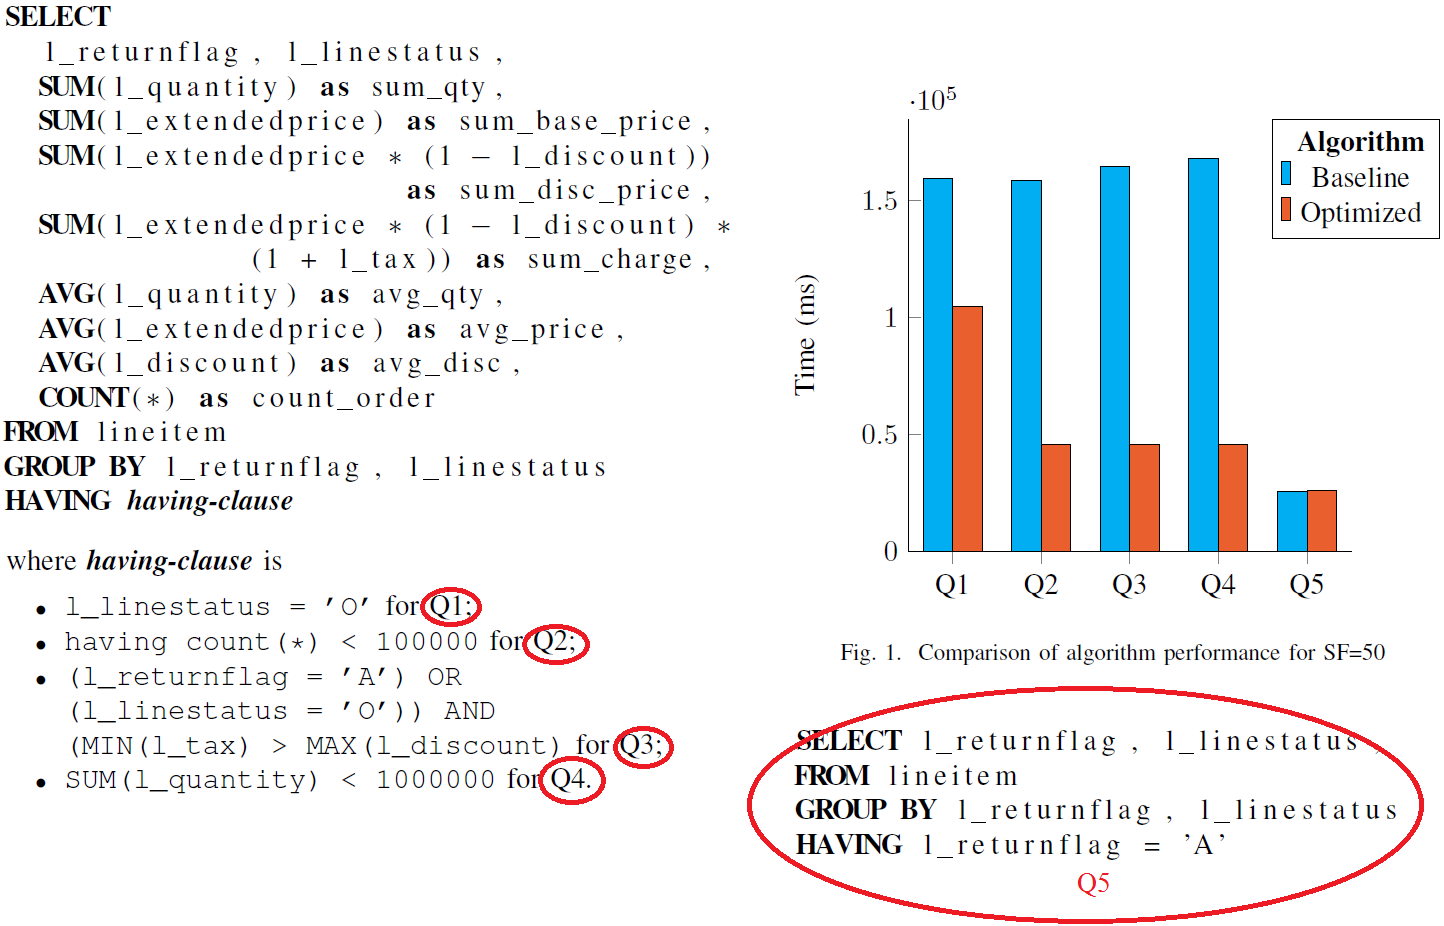
\includegraphics[width=0.95\textwidth]{./aggr-results}
	%\caption{A picture of the same gull looking the other way!}
\end{figure}
\end{frame}

\begin{frame}[fragile]
\frametitle{Window functions: syntax and concepts}
\begin{lstlisting}
window_function(column) OVER (
  [ PARTITION BY column [ , %*\ldots*) ] ]
  [ ORDER BY column [ ASC | DESC ] ]
  [ { ROWS | RANGE } BETWEEN %*\textit{frame\_start}*) AND %*\textit{frame\_end}*) ]),
\end{lstlisting}

\begin{columns}
	\begin{column}{0.5\textwidth}
		\noindent where \texttt{\textit{frame\_start}} may be
		\begin{itemize}
			\item \texttt{UNBOUNDED PRECEDING}
			\item \textbf{\textit{offset}} \texttt{PRECEDING}
			\item \texttt{CURRENT ROW}
		\end{itemize}
		
		\noindent and \texttt{\textit{frame\_end}} may be
		\begin{itemize}
			\item \texttt{CURRENT ROW}
			\item \textbf{\textit{offset}} \texttt{FOLLOWING}
			\item \texttt{UNBOUNDED FOLLOWING}
		\end{itemize}
	\end{column}
	\begin{column}{0.5\textwidth}
		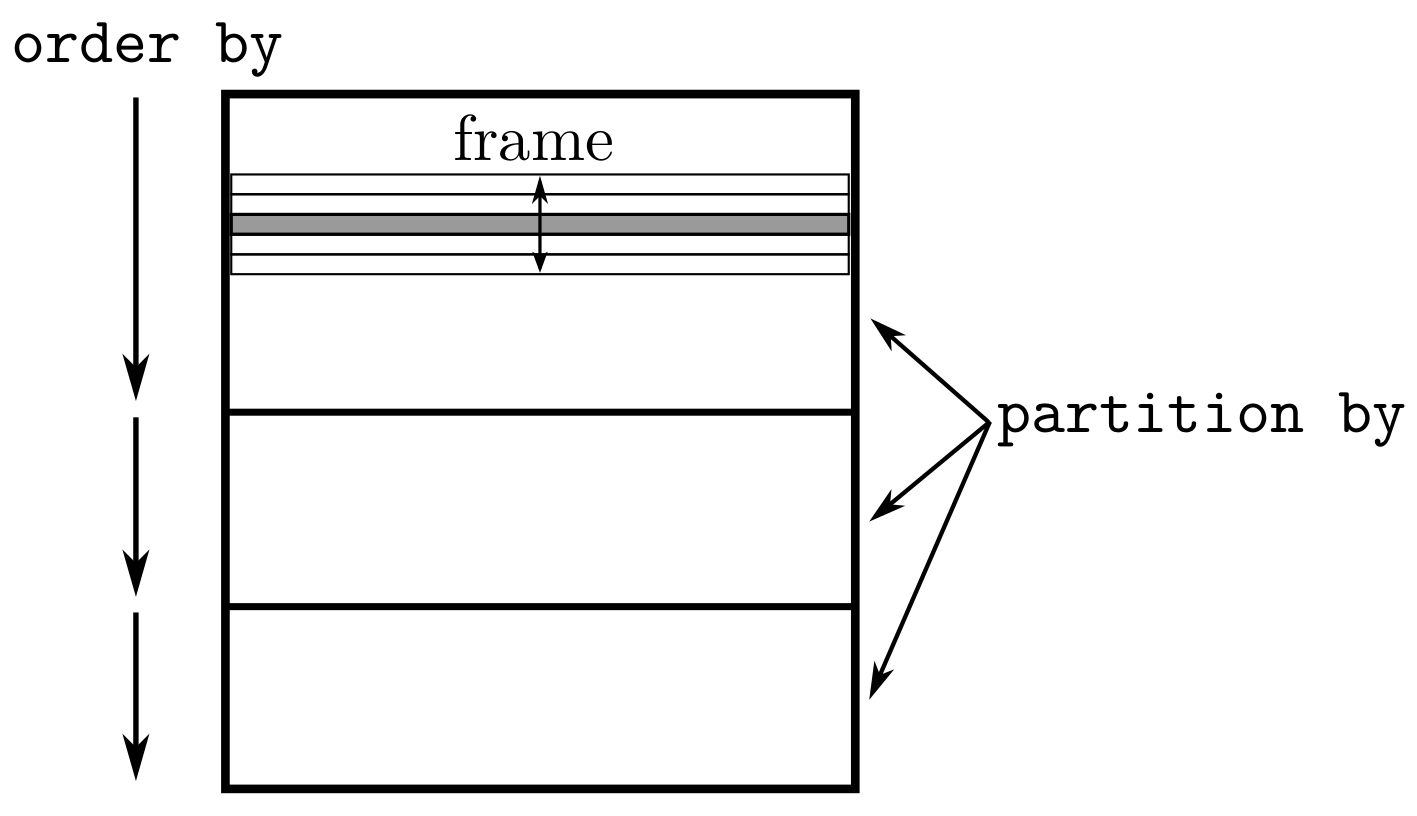
\includegraphics[width=1.0\textwidth]{wf_concepts}
	\end{column}
\end{columns}
\let\thefootnote\relax\footnotetext{Image is taken from the paper ``Efficient Processing of Window Functions in Analytical SQL Queries'' of Viktor Leis et al., VLDB, 2015}
\end{frame}

\begin{frame}{Window functions: processing strategies}
	\begin{itemize}
		\item Partitioning
		\begin{itemize}
			\item using hash table
			\item using sorting (can be combined with ordering)
		\end{itemize}
		\item Ordering
		\begin{itemize}
			\item separate for each group
		\end{itemize}
		\item Evaluation
		\begin{center}
			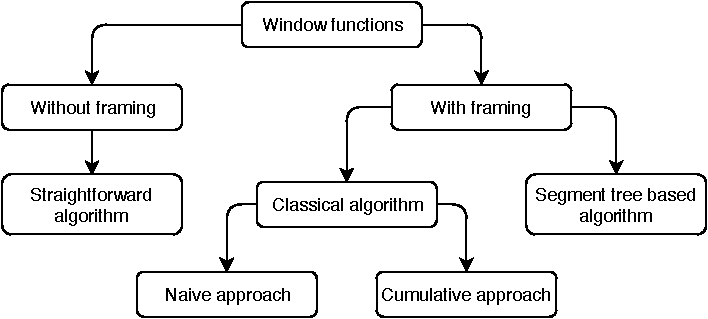
\includegraphics[width=0.7\textwidth]{window_functions_processing.pdf}
		\end{center}
		
	\end{itemize}
\end{frame}

\begin{frame}{Window functions: our contribution}
    \begin{itemize}
        \setlength\itemsep{1em}
        \item Considering possible materialization strategies and memory consumption models for them
        \item Segment tree generalization
        \item Segment tree application for evaluation of \texttt{RANGE}-based window functions
    \end{itemize}
    
    \let\thefootnote\relax\footnotetext{Details can be found in the paper ``Implementing Window Functions in a Column-Store with Late Materialization'', available at \scriptsize{\url{https://link.springer.com/chapter/10.1007\%2F978-3-030-32065-2_21}}} 
\end{frame}


\begin{frame}{Intermediate results caching}
    \begin{figure}
        \centering
        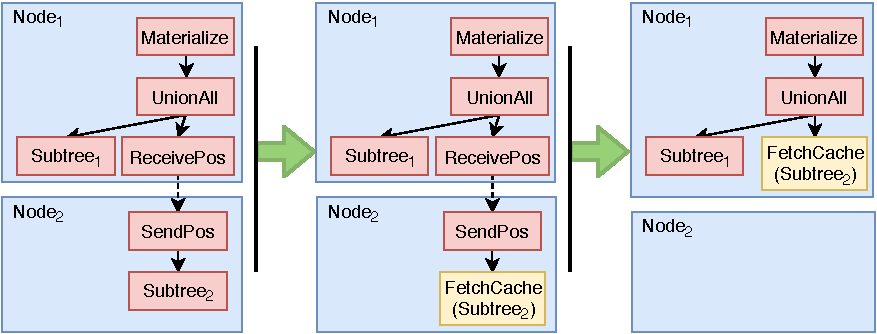
\includegraphics[width=\textwidth]{images/caching_v2.pdf}
    \end{figure}
    \begin{itemize}
        \item Before materialization; only positions are stored
        \item Intermediates are stored in-memory
        \item Allows compression of stored results to reduce memory footprint
    \end{itemize}
\end{frame}

\begin{frame}[fragile]{Intermediate results caching: the main idea}
    \begin{lstlisting}[language=C++]
struct QueryDescription {
    set<Partition> partitions;
    set<pair<Column, Column>> joins;
    set<ConstPredicate> const_predicates;
    set<ValueList> specific_values;
    Buffer plan;

    bool contains(const QueryDescription &other);
    double complexity();
    size_t expectedBlocks();
};
    \end{lstlisting}
    \begin{enumerate}
        \item Reduce every subplan to a descriptive structure
        \item Keep track of $N$ last queries
        \item Estimate every result's benefit as a function of computational complexity and size
    \end{enumerate}
\end{frame}

\begin{frame}{Intermediate results caching: performance}
    \begin{figure}
        \centering
        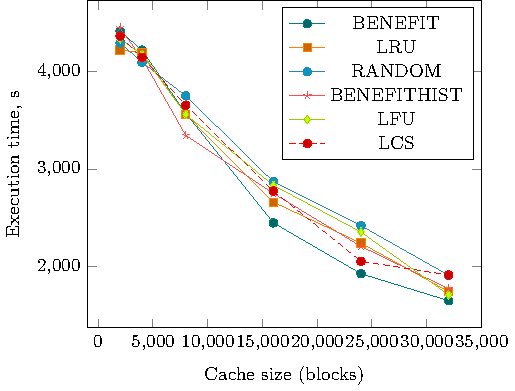
\includegraphics[width=.89\textwidth]{images/caching_performance.pdf}
    \end{figure}
\end{frame}



\begin{frame}{Our team}
Current members:

\begin{itemize}
    \item Viacheslav Galaktionov
    \item Valentin Grigorev
    \item Evgeniy Klyuchikov
    \item Kirill Smirnov
    \item George Chernishev
    \item Nadezhda Mukhaleva
\end{itemize}

Ex-members:

\begin{itemize}
    \item Anastasia Tuchina
    \item Evgeniy Slobodkin
\end{itemize}

\end{frame}

\begin{frame}{System State: 2017 $\longleftrightarrow$ 2018 $\longleftrightarrow$ 2019}

Technology stack: C++17, Git, Google Test, JSON, PostgreSQL (for result verification)

%\begin{center}		
%	\begin{tabular}{| l | r | r | r |}
%		\hline
%		Characteristic & 2017      & 2018 \\ \hline     \hline
%		Size           & 824 KB    & 1252 KB\\ \hline
%		Lines of code  & 11.5K     & 17.8K \\ \hline
%		Classes        & 116       & 198 \\ \hline
%		Modules        & about 75  & about 100\\ \hline
%		Tests          & about 80  & about 200\\ \hline	
%		Commits        & 800+	   & 1326? \\ \hline
%		Branches       & several   & about 30 \\ \hline 
%	\end{tabular}
%\end{center}

\begin{center}
	\begin{tabular}{| l | r | r | r |}
		\hline
		Characteristic & 2017      & 2018       & 2019       \\ \hline     \hline
		Size           & 824 KB    & 1252 KB    & 2100 KB    \\ \hline
		Lines of code  & 11.5K     & 17.8K      & 28.4K      \\ \hline
		Classes        & 116       & 198        & 366        \\ \hline
		Modules        & about 75  & about 100  & 185        \\ \hline
		Tests          & about 80  & about 200  & about 300  \\ \hline
		Commits        & 800+      & 1300+      & 1600+      \\ \hline
	\end{tabular}
\end{center}

			


\end{frame}



\begin{frame}{Future plans}

\begin{itemize}
\setlength\itemsep{0.5em}
\item Extending class of supported queries, move towards TPC-H and TPC-DS support;
\item Query optimizer;
\item Query adaptivity;
\item Compression support;
\item Technical stuff: REPL, visualization, parser (partially completed now)
\item ...
\end{itemize}
\end{frame}


\end{document} 
